%%%%%%%%%%%%%%%%%%%%%%%%%%%%%%%%%%%%%%%%%%%%%%%%%%%%%%%%%%%%%%%%%%%%%%%%%%%%%%%%
% This is the Mamba user manual Tex source

\documentclass[a4paper,10pt,oneside]{article}
\usepackage[table]{xcolor}
\usepackage{mamba}

%\renewcommand{\refname}{\vskip -24 pt}

\title{Mamba Image User Manual}
\author{Nicolas BEUCHER \and Serge BEUCHER}
\date{\today}

%%%%%%%%%%%%%%%%%%%%%%%%%%%%%%%%%%%%%%%%%%%%%%%%%%%%%%%%%%%%%%%%%%%%%%%%%%%%%%%%
% Tip and warning boxes environments
\definecolor{lightblue}{RGB}{220,220,255}
\newenvironment{tipBox}
{
    \begin{center}
    \begin{tabular}{ | b{0.1\textwidth} b{0.8\textwidth} | }
    \hline
    \rowcolor{lightblue}
    
\includegraphics[width=0.1\textwidth]{Crystal_Clear_action_info.png} &
}
{
    \\
    \hline
    \end{tabular}
    \end{center}
}

\newenvironment{warnBox}
{
    \begin{center}
    \begin{tabular}{ | b{0.1\textwidth} b{0.8\textwidth} | }
    \hline
    \rowcolor{yellow}
    
\includegraphics[width=0.1\textwidth]{Crystal_Clear_app_error.png} &
}
{
    \\
    \hline
    \end{tabular}
    \end{center}
}

%%%%%%%%%%%%%%%%%%%%%%%%%%%%%%%%%%%%%%%%%%%%%%%%%%%%%%%%%%%%%%%%%%%%%%%%%%%%%%%%
% Document

\begin{document}

\mambaCover
\mambaContent

\section{Introduction}

This document is the user manual of the library for Python \emph{Mamba Image}.

Mamba Image is a mathematical morphology library, its name actually stands for 
\emph{MA}thematical \emph{M}orphology li\emph{B}r\emph{A}ry \emph{Image} 
(For sake of simplicity, the library will be referred to as Mamba). The library 
provides a wide set of functions needed to perform common operations used in 
mathematical morphology like erosion, dilation, etc... but also more complex ones
(geodesic operators, watershed transformations...).

Before reading this document, make sure you have basic knowledge of Python
programming language (see the Python tutorial at 
\url{http://docs.python.org/tutorial/}) and that you know the basics of 
mathematical morphology (online courses are available at 
\url{http://cmm.ensmp.fr/~serra/acours.htm} and \url{http://cmm.ensmp.fr/~beucher/publi.htm}).

This document addresses various points to help you understand how to use and
enjoy Mamba, such as getting familiar with it, what it does and doesn't,
understand how the library works, what you can do to optimize it for your
needs. If you are new to it, read the next section, quick start, before going
further.

\pagebreak

\section{A quick start}

For all intent and purpose, we will now assume that you know what mathematical
morphology is, at least theorically (and your interest in Mamba is to go 
practical), and that you have a minimum know-how in programming with Python.

We are aware that fulfilling these two conditions may be quite difficult. It is 
likely you know one and not the other. The present authors were unable to 
fulfil them when the project Mamba started. So don't get discouraged if you are
not yet familiar with one aspect or the other. There is plenty information over
the web to get you started on either one. This document is not intended to serve
as a mathematical morphology course nor as a programming lesson as these goals are
beyond our time or ability to perform. However, we list at the end of the
document (see appendix \ref{cha:to_go_further}) various websites or pdf documents which are 
accessible online that can provide you with this information. Of course, we hope that
Mamba will give you the incentive to learn one aspect or the other to solve
any image analysis problem you may have (see our examples in appendix 
\ref{cha:examples} at the end to see the possibilities offered by such a tool).

To get started with Mamba, you need to install some software on your PC. The 
most obvious one is Python. You can find Python at \url{http://www.Python.org}. 
Download version 2.6 or 2.7 and install it. Mamba does not support Python 3 at the
moment. Once Python is installed, you will need to download the lastest version
of the Python Imaging Library (namely PIL) at \url{http://www.pythonware.com/products/pil/}
or. if you prefer, its friendly fork (namely PILLOW) at \url{http://python-imaging.github.io/}.
You need to download the version corresponding to your version of Python (this
should be indicated in the name of the file). Again install it. On Linux, you may
have to install the Tkinter library if it was not provided with your Python
distribution (Windows users don't need to worry as it is part of the standard 
Python distribution they just installed). Finally download the Mamba library 
from \url{http://www.mamba-image.org} (as for PIL select the version corresponding
to your Python version) and install it.

\begin{tipBox}
The Python Imaging Library (PIL), used in the previous Mamba releases is more and more
out of date because of its lack of evolution and support since its latest release (1.1.7).
Fortunately, a recent friendly PIL fork named PILLOW has been released. Since Mamba release 1.1.3,
PIL or PILLOW can be equally used with Mamba, which recognises automatically which library is
installed. Therefore, we recommend to use PILLOW, especially if you are under Linux, as the latest
Linux distributions come with PILLOW instead of PIL.
\end{tipBox}

These instructions may not be interpreted in the same way depending on your 
system specification. If you need more information refer to section
\ref{cha:inst_comp}.

At this point your PC is now equipped with every piece of software it needs to
use Mamba, so let's get started.

First, we will show you how to launch Mamba and use it in your programs.
To use Mamba, simply type in your Python console:

\lstset{language=Python}
\begin{lstlisting}
from mamba import * 
\end{lstlisting}

This import only gives you access to some of the basic functions implemented in
the library and, as important as they are, they are not complete enough to allow
you to do the most basic and usual operations found in every mathematical
morphology algorithm. To import these operators, type:

\lstset{language=Python}
\begin{lstlisting}
from mambaComposed import *
\end{lstlisting}

This import gives you access to more usual operators (well, we can say that it
gives you access to \emph{all} the usual operators or at least we intent to).
It is likely that any of your programs will start with those two imports.

You can find more information regarding these two modules/packages in section 
\ref{cha:content}.

\begin{tipBox}
If you are using Windows, you can start more easily by clicking on the created
Mamba Shell shortcut in your start menu. It will launch an IDLE (the standard
Python shell on Windows) with preloaded mamba modules and packages and some 
default images created. If you are an IDLE user, this is the
recommanded way (see section \ref{cha:lim_restrict} for more information
regarding Mamba and IDLE).
\end{tipBox}

You now have all the tools offered in Mamba loaded on your computer and you are
ready to try your ideas. Obviously you have some image that you would like to
process, so naturally the very first step is to load it into your program.

\lstset{language=Python}
\begin{lstlisting}
# Replace the "path/to/your/image" by the correct path
im = imageMb("path/to/your/image")
\end{lstlisting}

At this point, you can manipulate your image using the reference im. For example,
you could try to get some information about this image:

\lstset{language=Python}
\begin{lstlisting}
# Printing the size of the image (width, height)
print im.getSize()
# Printing the depth of the image 
print im.getDepth()
\end{lstlisting}

The first thing you may notice is that the returned image size is not the actual
image size (as it is registered when you look into the image properties). For
performance sake, Mamba can only work with images that have a width multiple of 64
and a height multiple of 2. If not, the image is automatically padded. You can 
also notice that your image was put into a greyscale image (the second command 
returns 8 which means 8 bits per pixel, the image pixels can take 256 values, from 
0 to 255). This is the default behavior for Mamba.

Well, this is all interesting but it does not give you access to the primary
properties of an image i.e. how it looks like. To do so, Mamba gives you access to
an embedded image displayer. You can call it for every image you create.

\lstset{language=Python}
\begin{lstlisting}
im.showDisplay()
\end{lstlisting}

This should have created a window displaying your image. There is no color
obviously because your image was transformed into a greyscale image upon loading.

The display comes with lots of options and possibilities to help you visualize
your image. More information can be found in section \ref{cha:disp_im}.

Now you have loaded your image, you are displaying it and you have access to 
some of its properties but one image is insufficient so you will have to create
other images to store your computation, compare, etc ... At this point you can
create them with the same properties as image im:

\lstset{language=Python}
\begin{lstlisting}
# Creating other images
im1 = imageMb(im)
im2 = imageMb(im)
im3 = imageMb(im, 1)
\end{lstlisting}

Here we created 3 new images with the same properties as our original image im.
Thus im1, im2 and im3 will have the same size as im. im1 and im2 also share 
the same depth as im (i.e. 8 bits per pixels) whereas im3 was created with a 
binary depth (1 bit per pixel as specified by the second argument). There are many
possibilities for creating new images, refer to section \ref{cha:create_im} for
more details.

You can activate the display for all of them as well. A window will be created
for each.

Now to give you an idea of how to use the functions of Mamba, we will now show
you a small example using the created images above.

\lstset{language=Python}
\begin{lstlisting}
# 1 - Computing the gradient of image im and putting the result in im1
gradient(im, im1)
# 2 - Computing a small opening of image im and putting the result in im2
open(im, im1)
# 3 - Computing the gradient of im2 and putting the result in im2
gradient(im2, im2)
# 4 - Converting im1 into binary and putting the result in im3
convert(im1, im3)
\end{lstlisting}

As random as these examples are (they are here for the sake of demonstration),
you may have already noticed some points. Firstly, function names closely
match the mathematical operators they are implementing (We tried to respect this
rule as best as we could to make the code more understandable). Secondly, you can
use an image both as input and output in the same function (see number 2). Last
but not least, convert is not the best function to transform your greyscale image into
a binary version at least from a mathematical morphology point of view.

And by the way, if you happened to have activated the display for the result
images, you may have found that the operations were quite slow (although in these 
basic examples, they are not so slow...). Indeed the 
display is automatically updated for each operation. Of course, when there is
only one (such as for convert) this is quite transparent but many functions, 
e.g. gradient and open, are a mix of other basic functions for which there is
a display udpate for every call. Let us assure you that the delay is only a
consequence of display updates.

\lstset{language=Python}
\begin{lstlisting}
# Activating the display and performing a size 100 erosion
im1.showDisplay()
erode(im, im1, 100)
# Now disabling the display and doing the same operation
im1.hideDisplay() # <- you can also close the window or minimize it
erode(im, im1, 100)
\end{lstlisting}

This example ends this very simple introduction to Mamba. Of course it does not
cover everything you can do with Mamba nor gives you all the details to better
harness its capabilities. However, hopefully now you have a basic understanding 
of how the library works. For more precision, read section \ref{cha:using_mamba}.
Also note that this document does not list the functions offered in Mamba, you
will need to refer to the Python reference document or to the Python API
quick reference for a list and explanations.

\pagebreak

\section{Why/When use Mamba?}

Before going further in this document, let's see why you should use Mamba and, 
almost more importantly, when. It can be sum up in the following sentence:

Mamba is meant to be a fast and easy library for coding mathematical morphology 
algorithms.

What we meant here is that, if your main concern is to try new algorithms to 
address your mathematical morphology problems while not waiting all night long 
for your result to come out or worse not come out because you made a mistake, 
then Mamba is meant for you. However, if you are looking for a library to perform
image processing tasks like convolutions, contrast enhancers or likewise, you 
had better not using it (try PIL instead). And by the way, Mamba does not make 
coffee (sorry about that...).

To do so, Mamba low level library is coded in C with performance through
simplicity in mind. The Python wrapper purpose is to give you an interface to 
that library which is fast to code and easy to play with (no compilation required 
and interactive help). Another objective regarding Mamba code is to be as 
portable as possible. This means that if you need to port your algorithm to a 
specific system you can easily adapt the C code to it.

Regarding licensing, Mamba is released under X11 license (also known as MIT 
license), see section \ref{cha:License} for more information.

To conclude this, let us remind you that mambas are fast-moving land-dwelling 
snakes of Africa. Their bite (at least for the black mamba) is extremely deadly 
but we assure you that no harm may come to you using Mamba... Well it won't bite
you.

\pagebreak

\section{License}
\label{cha:License}

Here is a copy of the license of Mamba. This license is known as the X11 license
(also named MIT license).

\vspace{0.5cm}

\begin{minipage}[c]{0.8\textwidth}%
 {\small Copyright (c) <2009>, <Nicolas BEUCHER and ARMINES for the Centre de 
 Morphologie Math\'{e}matique(CMM), common research center to ARMINES and MINES 
 Paristech>}{\small \vspace{0.5cm} \par}

{\small Permission is hereby granted, free of charge, to any person
obtaining a copy of this software and associated documentation files
(the \textquotedbl{}Software\textquotedbl{}), to deal in the Software
without restriction, including without limitation the rights to use,
copy, modify, merge, publish, distribute, sublicense, and/or sell
copies of the Software, and to permit persons to whom the Software
is furnished to do so, subject to the following conditions: The above
copyright notice and this permission notice shall be included in all
copies or substantial portions of the Software.}{\small \vspace{0.5cm} \par}

{\small Except as contained in this notice, the names of the above copyright 
holders shall not be used in advertising or otherwise to promote the sale, use 
or other dealings in this Software without their prior written authorization.}
{\small \vspace{0.5cm} \par}

{\small THE SOFTWARE IS PROVIDED \textquotedbl{}AS IS\textquotedbl{},
WITHOUT WARRANTY OF ANY KIND, EXPRESS OR IMPLIED, INCLUDING BUT NOT
LIMITED TO THE WARRANTIES OF MERCHANTABILITY, FITNESS FOR A PARTICULAR
PURPOSE AND NONINFRINGEMENT. IN NO EVENT SHALL THE AUTHORS OR COPYRIGHT
HOLDERS BE LIABLE FOR ANY CLAIM, DAMAGES OR OTHER LIABILITY, WHETHER
IN AN ACTION OF CONTRACT, TORT OR OTHERWISE, ARISING FROM, OUT OF
OR IN CONNECTION WITH THE SOFTWARE OR THE USE OR OTHER DEALINGS IN
THE SOFTWARE. }%
\vspace{1cm}
\end{minipage}

\begin{warnBox}
Please note that this license does \textbf{\textsc{not}} cover documentation and
images found in source packages.
\end{warnBox}

\pagebreak

\section{Requirements}
\label{cha:Requirements}

To use Mamba, you will need:
\begin{itemize}
\item A computer running Linux or Windows. Mamba will run on all kind of 
processors. However, you have to verify if yours supports SSE2 instructions. If you
are not sure, install the version of Mamba without SSE2, please note this version
is very slow. See \url{http://en.wikipedia.org/wiki/SSE2#CPUs_supporting_SSE2}
for a list of compatible CPUs.
\item Python version 2.6 or later (At the moment the library does not support 
Python 3).
\item Python Imaging library (PIL or PILLOW) for your current version of Python.
\item Tkinter (normally comes with Python on Windows systems but you may need to
install it on Linux systems).
\end{itemize}

To compile or modify the sources, you will need:
\begin{itemize}
\item Python version 2.6 or later with the distutils package.
\item Python development headers (normally comes with Python on Windows systems 
but you may need to install them on Linux systems).
\item SWIG version 1.3.33 or later.
\item GCC version 4.3.0 or later (or its Windows version MinGW32).
\item  Under Windows, you may choose Microsoft Visual C++ Express 2008 (to 
compile you will then need the stdint.h header. You can find it at 
\url{http://msinttypes.googlecode.com/svn/trunk/stdint.h}. Copy it in the VC/include 
directory of your Visual C++ installation).
\end{itemize}
Compilation instructions are given in the next section or in the README file 
provided with the library.

Mamba works with all kinds of processors. The library takes also profit of 64-bit
processors. To enable the 64-bit mode, you will need a 64-bit Python installed 
on your computer (The 64-bit mode is only supported on Linux systems).

\pagebreak

\section{Installation/Compilation}
\label{cha:inst_comp}

Mamba can be compiled and installed on various platforms and systems.
Instructions vary between systems. This section presents the official ways
to compile and install Mamba on your system. The compilation, distribution and
installation are performed using the distutils package which is the standard
Python way to do it (see \url{http://docs.python.org/library/distutils.html}).

\begin{tipBox}
The setup scripts (setup.py, setup\_visualcpp\_SSE2.py and setup\_mingw32\_SSE2.py)
can be found in src/mambaApi. Reading them may be a good idea if you encounter
some difficulties. You can also edit them to fit your needs.
\end{tipBox}

\subsection{Windows XP/Vista/Seven/Eight 32-bit}

If you are only interested in installing and don't want to go through the bother
of compiling it, just pick up the installer on the website, launch it and 
follow the instructions.

To compile, make sure you have correctly installed the required tools (see section
\ref{cha:Requirements}) and that they appear in your PATH environment variable.
In particular, make sure that SWIG binary (swig.exe) and GCC binary (gcc.exe)
path are devoid of spaces as this may cause problems to the setup script.

\begin{enumerate}
\item Get the latest version of the source (package "Mamba.X.X.zip")
\item Extract it in your local directory
\item Open a command line window
\item Browse to the created directory "Mamba.X.X"
\item Browse to src/mambaApi
\item type (select the line depending on which version of Mamba you want to 
produce and the compiler you are using):

\texttt{python setup.py build\_ext build} (visual C++ no SSE2)\\
\texttt{python setup.py build\_ext -cmingw32 build} (mingw32 no SSE2)\\
\texttt{python setup\_visualcpp\_SSE2.py build\_ext build} (visual C++ with SSE2)\\
\texttt{python setup\_mingw32\_SSE2.py build\_ext -cmingw32 build} (mingw32 with SSE2)

\item You can then install it.

\texttt{python setup.py install}

\end{enumerate}

Alternatively, you can create the installer that will allow you to 
distribute more easily your own version of Mamba. Replace step 6 above by the 
following instruction:

\begin{enumerate}
\setcounter{enumi}{5}
\item type (select the line depending on which version of Mamba you want to 
produce and the compiler you are using):

\texttt{python setup.py build\_ext bdist\_wininst} (visual C++ no SSE2)\\
\texttt{python setup.py build\_ext -cmingw32 bdist\_wininst} (mingw32 no SSE2)\\
\texttt{python setup\_visualcpp\_SSE2.py build\_ext bdist\_wininst} (visual C++ with SSE2)\\
\texttt{python setup\_mingw32\_SSE2.py build\_ext -cmingw32 bdist\_wininst} (mingw32 with SSE2)

\end{enumerate}

The installer produced will be in the dist directory. If you are choosing this
way to create your own distribution of Mamba, you can also add two options to
your build instructions:

\begin{itemize}
\item On Windows, you can create a specific IDLE shell call for Mamba by making
the installer run the appropriate post install script. Just add this option
after the bdist\_wininst command:

\texttt{-{}-install-script=mamba\_post\_install.py}

\item You can also decorate your installer with the Mamba logo (or your own) by
adding the following option:

\texttt{-{}-bitmap=../../doc/style/mamba\_logo.bmp}

\end{itemize}

\begin{warnBox}
If you are a Windows user, we strongly recommend you to use Visual C++ 2008 
instead of MinGW32 when generating a SSE2 distribution of Mamba. Indeed some
functions are not compiled with SSE2 when using the MingW32 compiler because
of possible crash (in particular the build operator related functions). Thus
performance may be lower when compiling with MingW32.
\end{warnBox}

\begin{warnBox}
When installing Mamba on a Windows 7 system (either 32-bit or 64-bit) with the 
IDLE shell, you may experience the following error message at the end of the 
install process:

\emph{close failed in file object destructor}

\emph{sys.excepthook is missing}

If it is the case, you have to know that this message is harmless (nothing is
broken in the installation). Therefore, you can ignore it.
\end{warnBox}

\subsection{Windows XP/Vista/Seven/Eight 64-bit}

If you are running one of the above systems, you possibly are using the Python for
64-bit Windows version. If this is the case then you \textsc{\textbf{can't}} use
Mamba. Since it works on 64-bit Linuxes you may wonder why. There are various reasons 
for this, but the main one is that Mamba requires PIL which is not released
for these platforms. Apparently, 64-bit Windows have some particularities that
make it quite difficult to produce stable versions for them. Until this change,
Mamba will not be offered for 64-bit Windows running the 64-bit version of
Python.

However you \textsc{\textbf{can}} use Mamba on your system provided you install
the 32-bit version of Python (will run without problems). Then all the 
instructions given for 32-bit Windows apply.

\subsection{Linux 32-bit or 64-bit}

We do not provide installers for these platforms because of the wide range of
Linuxes existing that make it a very challenging task to perform. However,
compilation and installation is simple enough on these systems. Make sure
you have all the required tools (use your package manager, if you have one, to 
get them), then follow the instructions:

\begin{enumerate}
\item Get the latest version of the source (package "Mamba.X.X.zip")
\item Extract it in your local directory
\item Open a terminal
\item Browse to the created directory "Mamba.X.X"
\item Browse to src/mambaApi
\item type:

\texttt{python setup.py build\_ext build}

\item You can then install it.

\texttt{python setup.py install}

\end{enumerate}

Please note that if you are running a 32-bit Linux, the version compiled by the
previous line will be \textbf{without} SSE2. If you want it, replace the last 
two items by:

\begin{enumerate}
\setcounter{enumi}{5}
\item type (for a SSE2 version of Mamba on 32-bit Linuxes):

\texttt{python setup\_mingw32\_SSE2.py build\_ext build}

\item You can then install it.

\texttt{python setup.py install}

\end{enumerate}


\subsection{Other platforms}

If you are not running one the afore-mentionned systems but still want to try
Mamba, you will need to find how to do it on your own. Currently, we have only access to
these kind of systems and thus cannot provide you with instructions on how to do
it with others. However, the basic requirements and instructions will likely apply.
Try to look what the distutils package says about your system.

By the way, if you have installed Mamba on another platform (successfully!), please
share your knowledge with others. We will be happy to insert your procedure in this
user manual (and give you credits...).

\pagebreak

\section{Contents of the library}
\label{cha:content}

Let's have a look at what is installed with the library.

All the files can be found in the site-packages/ directory of your local
Python installation under the directory mambaIm.

\subsection{\_mambaCore.so/\_mambaCore.pyd}

This is the main C core code compiled into a library for Python (mambaCore.so on
Linux systems and mambaCore.pyd on Windows systems). This file contains all the
basic functions and image structures definitions used by Mamba to perform the 
various mathematical morphology operations.

\subsection{mambaCore.py}

This file is automatically created by SWIG. It is the direct interface to the C 
library. This file is not intended to be used directly by the users and thus is
not documented.

\subsection{mamba.py}

This is the main module of the Python Mamba library.
It provides classes, functions and utilities to perform computations in a simple
and user-friendly environnement.

The Mamba module has been designed to facilitate the development and debugging 
of your programs. The performance is known to be lowered due to display update.
However, it can be disabled and enabled at will allowing to suppress the 
performance overhead.

\subsection{mambaDraw.py}

This module provides a set of functions to draw inside the image. You can draw
lines, squares,...

\subsection{mambaExtra.py}

This module provides a set of functions to interact dynamically with a display
and to perform specific tasks. It gathers functions that will likely not be used on a
daily basis. They are here to help the programmer in some specific cases.

\subsection{mambaDisplay.py}

This module provides the functions and classes performing the display in Mamba.
Usually you will not need to use it directly (mamba.py calls it) but if you wish
to develop your own display, this will be your starting point (see 
\ref{cha:create_own_disp}).

\subsection{mambaUtils.py}

This module regroups functions that embed common but complex or long low level
operations to manipulate image data. This module is not intended to be used by
the users.

\subsection{mambaError.py}

This module provides error handling functions for Mamba. C functions return an 
error code that can be interpreted using this module. Exceptions are raised if 
an error occured. This module will most likely never be used by a regular 
programmer.

\subsection{package mambaComposed}

This package provides a set of modules containing basic (and less
basic...) functions of mathematical morphology. The functions all use the basic
functions found in mamba.py to perform more elaborated transformations.

\subsection{package mambaShell}

This package is a container for functions and modules that are needed to create
and operate an appropriate shell for Mamba. In particular, it contains demo
presentations.

\pagebreak

\section{Using Mamba}
\label{cha:using_mamba}
\subsection{Implicit working of the library}

Before giving you details regarding how to fully grasp the library, we would
like to give you details regarding the way it implicitly work. This section aims
at presenting some aspects that will always be present in Mamba but likely not 
explained nor talked about.

When we talk about an 'EMPTY' image or edge, this always means that pixels 
(inside or outside the image) take value 0. Thus an empty
image is an image where all the pixels are set to 0. On the opposite, the term 
'FILLED' is always associated with the maximum possible value of a pixel (which depends on 
the image depth).

All image pixels are stored with unsigned integers. This is true for binary,
greyscale and 32-bit images.

As a consequence of the coding rules applied to Mamba, functions image parameters
always begin with the input arguments and ends with the output arguments (This 
is a general rule and there may be some exceptions for particular functions).
Most of the time, images arguments are imIn when the image is an input and imOut
when it is the output of the function. When functions require arguments other than 
image arguments (scalar values, edge or grid settings, etc.), they are placed after 
the image arguments.

When functions accept input and output images, you can safely use the same image
for both and you will obtain the expected result. If the function cannot 
guarantee this, it will return an error.

\subsection{A word for 0.2 users}

If you already are a Mamba user (either with version 0.1 or 0.2), you may have 
already seen that the new version is not backward compatible. Scripts
and programs created with 0.2 will not work with the new version. This is a 
consequence of the various works that were launched to correct some of the 
problems and to give Mamba a more appropriate architecture.

Among the changes made, here is a list of the most significant:
\begin{itemize}
\item Python functions arguments order was reversed.
\item Python functions were renamed to shorten them.
\item Mamba now supports multiple image sizes in one session.
\item 32-bit images are now unsigned.
\item The word "border" has been changed to "edge".
\item Mamba modules import has been simplified.
\end{itemize}

\subsection{Importing the modules and packages}

To use Mamba, simply type in your Python console:

\lstset{language=Python}
\begin{lstlisting}
import mamba
\end{lstlisting}

This is the recommanded Python import method because it separates each module
you may use in its own name reference space. However this is quite painful
to work with when you are using Mamba in a console mode as all the function 
calls have to be preceded by

\lstset{language=Python}
\begin{lstlisting}
mamba.
\end{lstlisting}

So to avoid this, type:

\lstset{language=Python}
\begin{lstlisting}
from mamba import *
\end{lstlisting}

The later will give you direct access to the module functions and variables.

To access the more advanced functions of Mamba, import the mambaComposed package:

\lstset{language=Python}
\begin{lstlisting}
import mambaComposed
\end{lstlisting}

This package is composed of various modules which can be imported separately (as
was done in Mamba 0.2) but, as there are lots of cross-reference between the
modules, importing one of them will very likely ends in importing the whole
package.

As with the mamba module, you can import it like this:

\lstset{language=Python}
\begin{lstlisting}
from mambaComposed import *
\end{lstlisting}

However, please note that some function names in mambaComposed are more likely to
interfere badly with other Python packages, e.g. open and close functions. To 
avoid this, while not being forced to type mambaComposed. before each function 
name, the best way would be to import it via an alias to shorten its name:

\lstset{language=Python}
\begin{lstlisting}
import mambaComposed as mC
\end{lstlisting}

Actually, this shortcut is used in the different mambaComposed modules, therefore it 
is recommended to do so when using these functions in your own modules.

Other modules are provided with Mamba:

\lstset{language=Python}
\begin{lstlisting}
import mambaExtra
import mambaDraw
\end{lstlisting}

See section \ref{cha:draw_extra} for more information on these modules.

\subsection{Grid and Edge}

Grid and edge are important notions in mathematical morphology. Let us explain
how they are handled in Mamba. 

The grid defines the neighbourhood of each pixel in an image. There are two 
possible grids in Mamba: \textbf{hexagonal} or \textbf{square}. The 
\textbf{hexagonal} grid defines six neighbours for each pixel as can be seen in 
figure \ref{fig:hxgrid}. The \textbf{square} grid defines the usual eight 
neighbours for each pixel as in figure \ref{fig:sqgrid}.

\begin{figure}
\centering
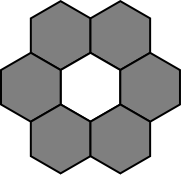
\includegraphics[scale=0.3]{hxGrid.png}
\caption{Hexagonal grid}
\label{fig:hxgrid}
\end{figure}

\begin{figure}
\centering
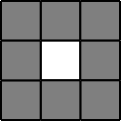
\includegraphics[scale=0.4]{sqGrid.png}
\caption{Square grid}
\label{fig:sqgrid}
\end{figure}

Be aware that the grid is never an image attribute, but a structuring element 
attribute. A structuring element is always defined on a given grid. Therefore, 
when performing a transformation with a given structuring element, the corresponding 
grid will be used with the image. Changing the grid of an image can be seen as a 
simple shift of the even lines of the image versus the odd ones so that the pixels 
belonging to an even line are between the pixels of the following odd line. The even 
lines are shifted to the right compared to the odd ones (the first line is numbered 0, 
it is therefore an even one).

The edge defines the status of all the pixels which are not in the image. Let us 
explain what this assertion means. Obviously, any image is made of a finite set 
of pixels. However, mathematical morphology operations, which are neighbourhood 
operations, need that the status of the neighbour points of the pixels which are at 
the edge of the image be defined, otherwise it would not be possible to define the 
transformation. This is the purpose of the edge attribute. The edge defines the 
virtual pixels which are outside the image. The edge (remember, it is the outside 
edge) can be set to \textbf{empty} or 
\textbf{filled}. The \textbf{empty} edge is assuming that external world surrounding 
the image is made of virtual pixels at value 0 (the edge is set to 0) whereas 
the \textbf{filled} edge assumes an external world completely filled 
(the edge is set to the maximum possible value of a pixel according to the image 
depth). 

By default, when it is launched, Mamba uses the \textbf{hexagonal} grid (through 
the DEFAULT\_GRID variable). Each function requiring a grid configuration as a parameter is 
given DEFAULT\_GRID by default. When an edge status is needed, the default
value is selected depending on the operator in use. The edge, as the grid, is not 
an image attribute.

There are different ways to change the grid. Firstly, you can use the setDefaultGrid 
function:

\lstset{language=Python}
\begin{lstlisting}

# Changes the default grid (DEFAULT_GRID) to HEXAGONAL
setDefaultGrid(HEXAGONAL)

# Changes the default grid (DEFAULT_GRID) to SQUARE
setDefaultGrid(SQUARE)
\end{lstlisting}

Secondly, you can do nothing and let some functions do the job for you!

As you will see later in this document, some functions need a direction or a 
neighbor as input. Figures \ref{fig:hxgriddir} and \ref{fig:sqgriddir} give you
the direction/neighbor encoding depending on the grid in use. The directions
are numbered from 0 to 6 or 8.

\begin{figure}
\centering
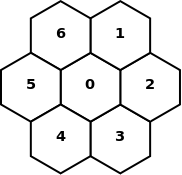
\includegraphics[scale=0.3]{hxGriddir.png}
\caption{Directions on hexagonal grid}
\label{fig:hxgriddir}
\end{figure}

\begin{figure}
\centering
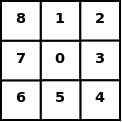
\includegraphics[scale=0.4]{sqGriddir.png}
\caption{Directions on square grid}
\label{fig:sqgriddir}
\end{figure}

You can get a list of all the available directions given the grid that is in use
by calling the function getDirections.

\lstset{language=Python}
\begin{lstlisting}
# Returns a list of all the available directions for the default grid
directions = getDirections()
# Returns a list of all the available directions for the SQUARE grid
directions = getDirections(SQUARE)
# Returns a list of all the available directions for the HEXAGONAL grid
directions = getDirections(HEXAGONAL)
\end{lstlisting}

There are other utilities functions that are provided by Mamba to handle 
directions/neighbors. Refer to the Python API reference.

\subsection{Creating and manipulating images}
\label{cha:create_im}

\paragraph{Creating images}

To handle images, a Python class named imageMb has been created. This class will allow
you to create, load, save and perform standard operations on your images.

The imageMb constructor offers a wide range of possibilities to create an image. 
Here is the list of all these possibilities:

\begin{itemize}
\item \texttt{\textbf{imageMb()}}: without arguments will create an empty 
greyscale image.
\item \texttt{\textbf{imageMb(im)}}: will create an image using the same size 
and depth than 'im'.
\item \texttt{\textbf{imageMb(depth)}}: will create an image with the desired
'depth' (1, 8 or 32).
\item \texttt{\textbf{imageMb(path)}}: will load the image located in 'path'.
\item \texttt{\textbf{imageMb(im, depth)}}: will create an image using the same 
size than 'im' and the specified 'depth'.
\item \texttt{\textbf{imageMb(path, depth)}}: will load the image located in 
'path' and convert it to the specified 'depth'.
\item \texttt{\textbf{imageMb(width, height)}}: will create an image with size 
'width'x'height'.
\item \texttt{\textbf{imageMb(width, height, depth)}}: will create an image with
size 'width'x'height' and 'depth'.
\end{itemize}

When not specified, the width and height of the image will be set to 
256x256. The default depth is 8 (greyscale).

For performance sake, Mamba works only with images that have a width multiple of
64 and a height multiple of 2. It means that if you requested the creation of
an image of size 360x201, Mamba will actually create an image of size 384x202. 
The actual image is always larger than or equal to the defined size.

There is a size limitation when you define images. This limitation is given by
the number of pixels in the image which must be lower than or equal to $2^{32}$.
This is a really huge value which allows you to define 65536x65536 images for instance.
A 200000x10000 image is also allowed (number of pixels lower than the limit).
Note however that, in practice, the real allowed maximum size is smaller as you would
need a fairly huge amount of memory to handle these images in Mamba. So, be sure
that your memory space is sufficient if you intend to use big images.

When loading an image from a file, please note that Mamba accepts all 
kinds of images (actually all the PIL supported formats). You can specify
the RGB filter that will be used to convert color image into greyscale 
image by adding the rgbfilter=<your\_filter> to the argument of the
constructor (see PIL documentation for examples of filters).

Example of image creation can be seen in the appendix \ref{cha:examples}.

\begin{tipBox}
Mamba allows you to create images with different sizes but not to perform
computations between them. If you want to do so, you will have to use the
cropCopy() function to extract the part of the images you want to match.
\end{tipBox}

\paragraph{Saving and loading images}

Once you have created an image and performed some operations on it, you may want 
to save it into a file. The imageMb class provides the method save() to do so:

\lstset{language=Python}
\begin{lstlisting}
# Saving the content of im1 image in test.png
im1.save('test.png')
\end{lstlisting}

The method uses PIL functions to save the image. Thus the format (bmp, gif, 
jpeg, ...) is automatically deduced from the extension used.

If you want to load an image into your imageMb object (assuming you did not make
it at the image creation) you can use the method load() to do so:

\lstset{language=Python}
\begin{lstlisting}
# Loading the content of test.png in image im1
im1.load('test.png')
\end{lstlisting}

Loading an image after the creation will not change the size of the original 
image to adapt it to the loaded image. The loaded image is padded/cropped to fit
the original size.

\paragraph{Other imageMb methods}

Besides creating, loading or saving your image, a range of other functionalities
are accessible using specific methods.

If you need to convert an image into another format (another depth), use the 
convert() method. Supported conversions are binary to greyscale (1->8) or 
greyscale to binary (8->1). A binary image is converted to a greyscale image using
0 for false and 255 for true. A greyscale image is converted to binary using the
following method: every pixel that is equal to 255 is set to true, otherwise 
false. convert() takes the required depth as argument. This method is here for 
convenient purposes, there are more elaborated ways to convert an image provided
inside Mamba.

\lstset{language=Python}
\begin{lstlisting}
# Converts the greyscale image into binary format
greyscale = imageMb(depth=8)
greyscale.convert(1)

# Converts the binary image into greyscale format
binary = imageMb(depth=1)
binary.convert(8)
\end{lstlisting}

If you want to erase an image, you can use the reset() method. 

\lstset{language=Python}
\begin{lstlisting}
# Erase the image im1 by setting all its pixels to 0
im1.reset()
\end{lstlisting}

The fill() method allows you to set all the pixels of an image to a given value.

\lstset{language=Python}
\begin{lstlisting}
# Fill im2 image with the value 3
im2.fill(3)
\end{lstlisting}

There are other methods that will be explained more thoroughly in the next sections.

\subsection{Pixels manipulation}

The imageMb class offers three methods to set or get pixels in the image.

\lstset{language=Python}
\begin{lstlisting}
# Setting the pixel at x,y in im2 to value
position = (x,y)
im2.setPixel(value, position)
# Same as previously but this method will not update the screen
im2.fastSetPixel(value, position)
# Getting the pixel value at position
value = im2.getPixel(position)
\end{lstlisting}

\subsection{Color palette}

Color palette defines the way a grey pixel will be converted to color. It 
associates for each possible value (0-255) a tuple of values describing the red, 
green and blue components (R, G, B) of the wanted color. The final palette is 
built by concatenating all these tuples into a single one.

Mamba comes with three predefined palettes:

\lstset{language=Python}
\begin{lstlisting}
# The rainbow colors (0 equals black)
rainbow

#The inverted rainbow colors (0 equals white)
inverted_rainbow

#The patchwork colors (0 equals black), used mainly to
#better visualise mosaic images
patchwork
\end{lstlisting}

You can see the results of using these palettes in figure \ref{fig:palette}.

\begin{figure}
\centering

\includegraphics[scale=0.3]{test_ramp.png}
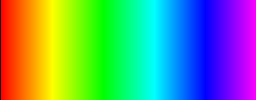
\includegraphics[scale=0.3]{test_ramp_r.png}
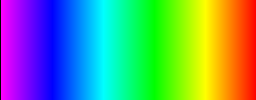
\includegraphics[scale=0.3]{test_ramp_ir.png}
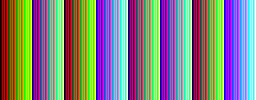
\includegraphics[scale=0.3]{test_ramp_p.png}
\caption{Effects of the rainbow, inverted rainbow and patchwork palettes on the first 
image}
\label{fig:palette}
\end{figure}

To apply or disable a palette to your image, use the following methods:

\lstset{language=Python}
\begin{lstlisting}
# Indicates that im1 will use palette as a color conversion
# table for display 
im1.setPalette(palette)

# Reset any palette conversion (the image will return to greyscale display)
im1.resetPalette()
\end{lstlisting}

When you apply a palette to an image, it will affect its display and the image 
stored by saving. The computations are not impacted. Be also aware that, if you 
save your image in color, you may have different values when reopening it with 
Mamba as the color to grey scale converter is not using your palette.

\subsection{Displaying images}
\label{cha:disp_im}

When trying new algorithms, it can be very useful to be able to follow the 
evolution of your images without having to save the image at each step. Mamba
provides a graphical interface, see figure \ref{fig:win}, which can display 
every required image into its own display window.

To activate a display, type:

\lstset{language=Python}
\begin{lstlisting}
# Shows the image im in its own window
im.showDisplay()
\end{lstlisting}

\begin{figure}
\centering
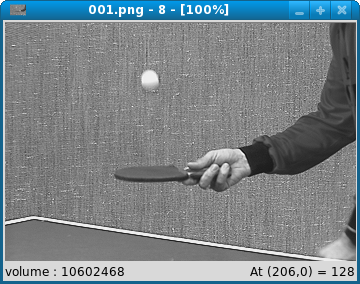
\includegraphics[scale=0.5]{mamba_win.png}
\caption{Image displayer window}
\label{fig:win}
\end{figure}

Every modification on this image will then be shown inside the opened window.
This operation is known to be very demanding on performance. The display also
gives information regarding the image volume, the position of the mouse inside
the image (and the pixel value associated).

There are numerous possibilities to control the display, here is the list of
keys and controls available inside the display:

\begin{itemize}
\item \textbf{Z and A}: These keys will respectively zoom in and out. You can
also control zoom using your mouse wheel.
\item \textbf{P}: will dynamically (de)activate the color palette (provided you
attach one to your image using the setPalette() method).
\item \textbf{<Control-V>}: will copy any image stored inside the clipboard 
in your image (only works on Windows platforms).
\item \textbf{<Control-F>}: will freeze/unfreeze the display. See freezeDisplay() 
method below.
\item \textbf{<Control-R>}: will reset the display to its original size and 
zoom value.
\item When zoom value allows it, you can grab the image using your mouse by
holding the left button down and moving it.
\end{itemize}

\begin{figure}
\centering
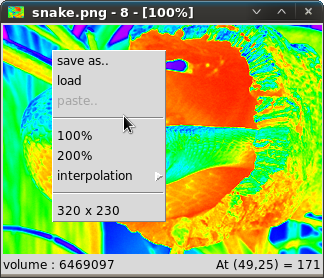
\includegraphics[scale=0.5]{mamba_menu.png}
\caption{Contextual menu}
\label{fig:menu}
\end{figure}

A contextual menu is also available by right-clicking in the display. It offers
services like saving, opening, etc. Figure \ref{fig:menu} shows an example of 
contextual menu. The first three choices are obvious. Then, you can choose a zoom
value between 100\% or 200\%. Interpolation is the way image will be processed
before being displayed when zoom value is different than 100\%. The choice
may affect the speed of display (for more information regarding the interpolation
methods, refer to PIL documentation). The last menu item indicates the size of
the image.

If you want to disable the display you have two options, either close the window
by clicking the appropriate button or type:

\lstset{language=Python}
\begin{lstlisting}
# Hide the window associated with im
im.hideDisplay()
\end{lstlisting}

Both operations will prevent the display to be updated for every modification of
the image and thus will remove the performance overhead (reducing or minimizing 
the display window will have the same result for performance but the window will
remain visible in your access bar).

If you want to stop the display from being automatically updated when a 
computation is performed while still being able to see it, you can freeze the 
display using the appropriate method:

\lstset{language=Python}
\begin{lstlisting}
# Freeze the window associated with im (no more updated)
im.freezeDisplay()

# Unfreeze the window associated with im (updated again)
im.unfreezeDisplay()
\end{lstlisting}

Sometimes, you will have lots of images opened and displayed making it quite
messy on your desktop and thus very difficult to read and analyze. There are a
bunch of methods and functions to help you organise your displays.

Firstly, you can give a name to your image that will be displayed in the window
title making it easier to know what is represented by the display:

\lstset{language=Python}
\begin{lstlisting}
# Setting im name to 'result'
im.setName('result')
\end{lstlisting}

When the screen gets filled with lots of displays it can be excruciatingly
boring and slow to order all of them so that they don't overlap. To make sure 
displays are properly and automatically organised you can call the following 
function:

\lstset{language=Python}
\begin{lstlisting}
tidyDisplays()
\end{lstlisting}

The function does not do miracles (like increasing your screen resolution) so
don't have too much expectations.

Large and small images are not displayed at their original size but they are
zoomed in (if they are too small) or zoomed out (if they are too large). By
default, images larger than 400 in width or height are zoomed out by a factor 2
until the size of the zoomed out displayed image is below this maximum value.
In the same way, an image smaller than 200 will be zoomed in (x2) until
the displayed image is larger than this minimum. For instance, a 1024x1024 image
will be displayed after a zoom-out equal to 25\% whereas a 200\% zoom-in will be
applied on a 128x128 image.

The default values of the display sizes can be changed by means of the following
functions:

\lstset{language=Python}
\begin{lstlisting}
setMaxDisplay(size)
setMinDisplay(size)
\end{lstlisting}

where size is a tuple containing the upper (in setMaxDisplay) or lower (in
setMinDisplay) limits of the width and height of the display.
These functions belong to the mambaDisplay module. It is wise to use them at
start before displaying any image. Under Windows, these functions could be put
in the \_init\_.py file of the Mamba shell (see section \ref{cha:mamba_shell}).

\lstset{language=Python}
\begin{lstlisting}
# Setting display max size to (800,800)
import mambaDisplay
mambaDisplay.setMaxDisplay((800,800))
\end{lstlisting}

\textbf{Important notice}: We saw previously that two grid definitions were 
available in Mamba: hexagonal or square grids. However, any image will always be 
displayed on a square grid, even if this image has been obtained with an operator 
defined on the hexagonal grid! Remember: the grid is an operator attribute, not an 
image attribute. This may lead to some strange phenomenons if you are displaying 
small hexagons for instance. They seem to be distorted and in fact they are. However, 
be sure that it's only a display artefact: the operator is really applied on an hexagonal 
grid (as you may ascertain this by displaying larger hexagons).

\subsection{Modules in mambaComposed}

mambaComposed is a Python package regrouping modules implementing the most 
common operators used in mathematical morphology based on standard Mamba 
functions.

Here is the complete list of modules found in mambaComposed, they are more or less
organised by families of operators:

\begin{itemize}
\item \textbf{erodil}: this module contains the erosions and dilations by elementary 
structuring elements (square, hexagon, segment, diamond, etc.) but also erosions 
and dilations by doublets of points, by dodecagons and octogons.
\item \textbf{erodilLarge}: this module contains erosion and dilation transformations 
with large structuring elements (large hexagons, squares, dodecagons and octogons). 
A specific implementation allows a dramatic speed enhancement of these operators.
\item \textbf{geodesy}: basic geodesic operators but also geodesic reconstructions 
(build and dualbuild) are available here.
\item \textbf{contrasts}: this module contains various contrast operators: morphological 
gradients and top-hat transformations.
\item \textbf{openclose}: various openings and closings are included in this module.
\item \textbf{residues}: this module contains some binary and greytone residual 
transforms (skeleton by opening, ultimate erosion, quasi-distance, ultimate opening,
etc.).
\item \textbf{filter}: some morphological filters are available in this module 
(alternate sequential filters, levellings).
\item \textbf{extrema}: this module provides a set of operators dealing with maxima and
minima of a function. New operators linked to the notion of dynamics are provided.
\item \textbf{partitions}: This module contains operators acting on partitions. These
operators may act on each cell of the partition independently, or they consider each cell
of the partition as a node of a weighted graph. Very powerful geodesic reconstructions and
labellings applied on partitions are also available in this module. 
\item \textbf{thinthick}: this module regroups general hit-or-miss transforms, thinnings 
and thickenings. Homotopic thinnings and thickenings (skeletons) are also included 
in this module.
\item \textbf{segment}: this module is devoted to segmentation tools. It contains 
mainly different variations of the watershed transformation.
\item \textbf{hierarchies}: More advanced segmentation operators mainly based
on hierarchical images (waterfall, P algorithm ...).
\item \textbf{sequence}: this module contains some operators applied on sequences. 
A sequence is a list of successive images, which can be considered as a 3D image.
\item \textbf{measure}: various measures are contained in this module. These measures 
are performed on binary images and the main ones are area, perimeter, connectivity 
number, diameters.
\item \textbf{statistic}: a few statistical measurements (mean, variance) are 
available here.
\item \textbf{miscellaneous}: this module gathers operators which do not belong to
any other category.
\end{itemize}

\subsection{Structuring elements}

The module erodil defines two of the most important operations of mathematical
morphology: erosion and dilation through functions erode and dilate respectively.
The mathematical definition of these operations is based on a structuring
element which controls the behavior of the operator.

The erodil module implements a class, named structuringElement that allows you to
describe a structuring element to be used with the erode and dilate functions. This
class can only describe structuring elements that are included in the local 
neighbors of the central point (adjacent points).

\begin{figure}
\centering
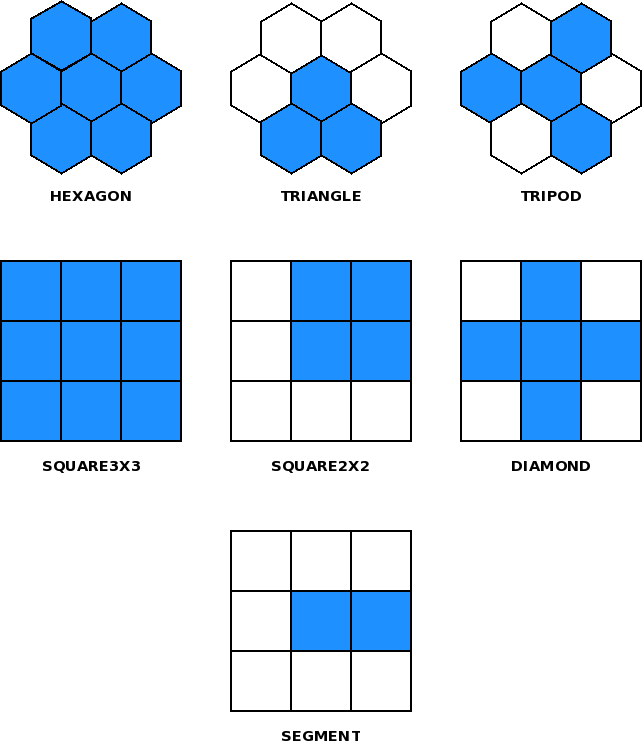
\includegraphics[scale=0.3]{se.png}
\caption{Structuring elements defined in Mamba}
\label{fig:se}
\end{figure}

Erodil already includes some of the most usual structuring elements. Figure
\ref{fig:se} gives their list and representation.

You can define your own structuring element easily. To do so you will need to
identify the grid it is based on and the points that you want to include 
inside your structuring element. Refer to figures \ref{fig:hxgriddir} and 
\ref{fig:sqgriddir} for neighbors coding values. Here is an example:

\lstset{language=Python}
\begin{lstlisting}
# Creating a reverse triangle
reverse_triangle = mambaComposed.structuringElement([0,1,6], mamba.HEXAGONAL)

# performing an erosion with the created structuring element
mambaComposed.erode(imIn, imOut, 1, se=reverse_triangle)
\end{lstlisting}

\begin{warnBox}
Some erosion and dilation functions implemented in Mamba do not use this
structuring element class for performance or feasability reasons.
\end{warnBox}

\begin{warnBox}
Be also aware that when you are combining operations using a structuring element
and operations using a grid you may have discrepancies between the structuring
element internal grid and the grid you used as an argument (or the default). To
prevent this, use the getGrid() method of the structuring element class.
\end{warnBox}

\subsection{Drawings and Extra}
\label{cha:draw_extra}

Two specific modules have been created to allow you to draw inside Mamba images
and to offer some extra display methods.

The module mambaDraw offers functions to draw various forms inside the image, 
e.g. lines, squares or boxes, and functions to extract information regarding pixel
values (intensity along a segment, ...).

The module mambaExtra offers functions to display, interact and generally 
perform operations that need the constant intervention of the programmer. For
example, this module provides an interface to allow dynamic threshold of a given
image (threshold value can then be modified on the fly by the user).

Both modules are described in the Python Reference document.

\subsection{Mamba Shell}
\label{cha:mamba_shell}

\textbf{Only on Windows}

The Mamba Shell is in fact a simple shortcut to IDLE, the standard Python shell
integrated into a Tkinter GUI. This shortcut serves three purposes:

\begin{itemize}
\item Make sure IDLE is started with the correct options to run properly Mamba
(see section \ref{cha:lim_restrict}.
\item Make it easy for beginners to start Mamba by providing them a shortcut
to a fully working environment with preloaded modules and packages.
\item Make it easy for advanced users to customize their default environment
(number of loaded images, size, particular imports ...) by editing an appropriate
file.
\end{itemize}

\begin{tipBox}
If you are not using IDLE as your Python environment, you can still benefit
from the mambaShell by simply importing it inside your own Python shell.
The syntax "from mambaShell import *" is strongly advised for easier use.
\end{tipBox}

\subsection{Regarding optimizations}

\begin{tipBox}
If you are trying to optimize your algorithm, the Python reference documents
will be useful to obtain information on how functions operate and what
sort of performance is to be expected. See section \ref{cha:other_docs}.
\end{tipBox}

Mamba is a very large library implementing a lot of functions. Consequently, it
is likely there is more than one way to create your algorithm using the functions
provided by the library. However, among all these possibilities, one is surely more
fitted to your purpose (as regards code clarity and comprehension, speed, size ...).

Regarding speed, you will likely have to study extensively the various
available functions. Mamba always tries to implement the fastest function to 
perform any task. However, sometimes other constraints (like readability and
simplicity) gets in the way of the fastest implementation.

For example, consider the opening by build of an image. The openByBuild function
found in the mambaComposed package is appropriate to perform this operation and
is as fast as possible if it has to work with all image depths indiscriminately.
This operator uses the build function (in mambaComposed) which works with any image
depth. However, there exists (im mamba.py package) a faster reconstruction operator,
hierarBuild, which works only with 8-bit images. Therefore, If you know that you are
only using greyscale images, it might be a good idea to create your own openByBuild
function like this:

\lstset{language=Python}
\begin{lstlisting}
import mambaComposed as mC
import mamba

def openByBuild_greyscale(imIn, imOut, n=1, se=mC.DEFAULT_SE):
    """
    Performs an opening by reconstruction operation on image 'imIn' and puts the
    result in 'imOut'. 'n' controls the size of the opening.
    
    This function only works for greyscale image and is an optimization of
    openByBuild.
    """
    
    imWrk = mamba.imageMb(imIn)
    mamba.copy(imIn, imWrk)
    mC.erode(imIn, imOut, n, se=se)
    mamba.hierarBuild(imWrk, imOut, grid=se.getGrid())
\end{lstlisting}

In other cases, Mamba will offer two functions performing the exact same 
operation with identical results but doing it with two algorithms presenting
different performance characteristics.

Consider the case of erosion using an hexagon. Two functions exist in Mamba to
perform this operation: erode and largeHexagonalErode.

\lstset{language=Python}
\begin{lstlisting}
# Erosion of imIn by an hexagon of size 1 put into imOut
erode(imIn, imOut, 1, se=HEXAGON)
largeHexagonalErode(imIn, imOut, 1)
\end{lstlisting}

In the example above, the result is the same for both functions. However, erode is
more than two times faster than largeHexagonalErode. But in this case:

\lstset{language=Python}
\begin{lstlisting}
# Erosion of imIn by an hexagon of size 20 put into imOut
erode(imIn, imOut, 20, se=HEXAGON)
largeHexagonalErode(imIn, imOut, 20)
\end{lstlisting}

largeHexagonalErode is this time more than two times faster than erode. You will
have to take into account this particularities when implementing your algorithm
if you want to speed it up. Regarding largeHexagonalErode, refer to section 
\ref{cha:opt_ero_dil} for more information.


\pagebreak

\section{Add-ons and extensions}
\subsection{mambaRealtime}

The Mamba Realtime module is an extension to the Mamba library for Python that 
allows you to test your algorithms on realtime acquired images.

The Mamba library allows you to develop easily and rapidly applications based on 
mathematical morphology algorithms. 

Most of the time, you will test and try your ideas on static images to make sure 
that your algorithm is working correctly and efficiently. However, as good as 
this approach might be, it still lacks something when you want to confront your 
algorithm to "dynamic real life situation", meaning noise, unpredictable 
movement, fast input, etc ... that your algorithm will have to handle to 
efficiently work in a realtime situation.

The Mamba Realtime was built to help you test these situations easily without 
having to recode your algorithm in another language.

Currently two versions of this module exist, one for Windows platforms and 
another for Linux platforms. It offers the following services :

\begin{itemize}
\item Acquire images from supported image acquisition device (Video 4 Linux 2
devices on Linux or DirectShow devices on Windows). Currently, this means that
most of the webcams are 
supported.
\item Retrieve images from video sources using the FFmpeg library (lots of video
codecs are supported).
\item Display the result of your algorithm in realtime.
\item Record the result using the FFmpeg library.
\end{itemize}

\begin{warnBox}
Please note that the Mamba Realtime module is \textbf{NOT} released under 
the same license. Currently this module is under GPL. Consult the appropriate
documentation for more information.
\end{warnBox}

For more information regarding this add-on, refer to the appropriate document.

\subsection{mamba3D}

The Mamba 3D package is an extension to the Mamba library allowing you to 
manipulate 3D images. It offers classes, methods and functions to store 3D images, 
to display them and to process them with operators and algorithms based on 
mathematcal morphology.

Mamba3D is meant as much as possible to work just like Mamba. If you are
familiar with Mamba you will have no trouble transferring your algorithms in
a 3D context. However, it is still recommended to read the specific user manual
of this extension because some elements differ between Mamba and its 3D
extension.

\pagebreak

\section{Limitations and restrictions}
\label{cha:lim_restrict}

Unfortunately, Mamba has some built-in limitations that may be corrected later
but that you will have to deal with in the meantime.

Whatever image you load, it will always be assumed that it is a greyscale image.
By default, Mamba uses the ITU-R 601-2 luma transform to convert color images 
into greyscale images. You can of course specify your own transformation matrix 
(refer to the Python and PIL reference documentations).

Mamba is known to have some troubles with IDLE. Mamba uses
Tkinter for image display and this may produce interferences with IDLE. The
problem is known to occur when IDLE is run with subprocess enabled which is the
default mode when IDLE is invoked through the Windows main menu. However, there 
is no problem when IDLE is started with no subprocess (option -n) as, for 
example, when right-clicking on a Python file and selecting "Edit with IDLE" from
the contextual menu. IDLE will display a short sentence if subprocesses are
deactivated before the first shell prompt. So if you want to use IDLE, you have
three options:

\begin{itemize}
\item Start IDLE with subprocess disabled (option -n). This will allow you to 
use Mamba display but unfortunately will prevent you using the integrated
debugger. The Mamba Shell on Windows is in fact a shortcut to do this.
\item Start IDLE with subprocess enabled (default mode on Windows) but do not
use Mamba standard display. This way you have access to the integrated debugger.
\item Install Mamba with the IDLE shell and launch MambaShell at startup (see
section \ref{cha:mamba_shell}).
\end{itemize}

In any case, Mamba should work perfectly with the standard Python shell 
(command line).

Along those problems with IDLE, you can also face difficulties when using
Mamba with other GUI libraries. Indeed, when using the embedded display,
Mamba relies on the PyOS\_InputHook trick. It allows the Python shell (where 
you type all your commands) to still be operational while at the same time
processing GUI events (such as mouse clicks keyboard inputs ...). When you
start any Mamba display, Tkinter grabs the hook thus making it unavailable
for other libraries which might need it. Similarly if Mamba is started
after a library that has grabbed the hook, the embedded display will not
work (display will be frozen). In particular, if you are a user of pylab,
make sure to import it \textit{after} Mamba because it is likely
this library will grab the hook (you must do this only if your intention is to
display Mamba images). It is not sure we will be able to fix this in a near
future. However, as long as you don't need to use the display, Mamba should 
work fine with any other library.

\pagebreak

\section{Other documents}
\label{cha:other_docs}

Mamba documentation is pretty large and covers C API, Python API, user manual 
and add-ons documentation. Here is a list of these documents and what 
information you can find in them:

\begin{itemize}
\item \textbf{\textsc{mambaApi Reference Manual}}: This document refers to the
low-level C API. It is generated using sources code and Doxygen. If you intend 
to modify the C functions, this document may be useful to you. It gives some
explanations regarding the image data structure used inside Mamba. Have also
a look at section \ref{cha:lib_arch} for general information regarding Mamba
architecture.
\item \textbf{\textsc{Mamba Image Library Python Reference}}: As soon as you
start using Mamba, you will need to keep this document close to you. All the
Python functions present in Mamba are explained in this document. It gives
information on how to use them, what sort of result to expect and so on... 
\item \textbf{\textsc{Python API quick reference}}: This document is the very
compacted version of the previous one. All the functions listed on the shortest
possible number of pages plus some of the more useful pieces of information you
might need. This quick reference is meant to help you quickly remember function
name and arguments but it can also be useful to get to know all the functions
implemented in Mamba.
\item \textbf{\textsc{Mamba Image Library Coding Rules and Standards}}: This
document describes various rules which should be enforced when programming new
functions and operators in Mamba. It indicates also some good practices that
should avoid problems in your daily use of Mamba. Obviously, these rules are not
compulsory. However, we strongly advise you to follow them if you intend to share
your operators and functions with others.
\end{itemize}

\pagebreak

\section{Algorithmic approaches in Mamba}

Some of the operators included in Mamba are based on specific algorithms.
In this section, we list some of them and give references to the articles or 
courses that describe them. You can also take a glimpse inside the sources to
see how they were implemented.

\subsection{Hierarchical lists : Watershed and Build}

Mamba is using hierarchical lists to perform watershed computations and some
particular build operators.

The use of hierarchical lists for watershed was first described in a patent 
document. This article described mainly an algorithm to extract basins.

\begin{enumerate}
\setcounter{enumi}{0}
\item \label{art:meyer} Fernand Meyer,
\emph{Image processing method by hierarchical queues},
Available at \url{http://www.freepatentsonline.com/EP0576584.html}, 1992
\end{enumerate}

More details for a similar algorithm allowing to extract an idempotent 
watershed line can be found in the following article.

\begin{enumerate}
\setcounter{enumi}{1}
\item \label{art:beucher2} Serge Beucher, Nicolas Beucher,
\emph{Hierarchical queues implementation: general description and enhancements
in Mamba software library},
Available at \url{http://cmm.ensmp.fr/\~beucher/Mamba\_documentation.html},
(to be published)
\end{enumerate}

Mamba implements these algorithms in the C core library for performance sake.
If you are interested, you can find them in the sources in files:

\begin{itemize}
\item \textbf{mambaApi\_loc.h}: The data structures used to represent the 
hierarchical lists in Mamba are described in this file.
\item \textbf{MB\_Basins.c}: A simple implementation of the hierarchical queues
to extract basins using a marker image for flooding wells. This is the simplest
use of hierarchical lists that is done in Mamba.
\item \textbf{MB\_Watershed.c}: An implementation of the hierarchical queues to
extract basins and watershed lines using a marker image for flooding wells.
\end{itemize}

Build (and its dual) operation can be performed using hierarchical queues in
Mamba by calling the appropriate functions. The implementation refers to
\ref{art:beucher2}.

Here is the list of source files implementing these operators. They are based on
the same data structures for the hierarchical lists as watershed operators:

\begin{itemize}
\item \textbf{MB\_HierarBld.c}: Implementation of the build operator for
greyscale images using the hierarchical lists.
\item \textbf{MB\_HierarDualBld.c}: Implementation of the dual build operator
for greyscale images using the hierarchical lists.
\end{itemize}

\subsection{Labeling}

The labeling algorithm implemented in Mamba employs a version of the union-find 
algorithm.

\begin{enumerate}
\setcounter{enumi}{2}
\item \label{art:wikipedia} Wikipedia Free Encyclopedia, 
\emph{Connected component labeling},
Available at \url{http://en.wikipedia.org/wiki/Connected\_Component\_Labeling}, 2007
\end{enumerate}

\begin{warnBox}
The label operator in Mamba is controlled by two parameters, lblow and lbhigh, set to
1 and 256 respectively. Note that, with this default setting, label values multiple of 256
(256, 512, etc.) are not used in the labelling. This is true whatever the lblow and lbhigh
settings. Be aware of this charecteristic when using the label operator! More generally,
modifying lblow or lbhigh (in the range [1,255] for lblow and [2,256] for lbhigh) prevents
the use of all the values modulo 256 which are not in the range [lblow, lbhigh-1].
\end{warnBox}

The code source implementing this algorithm can be found in the C core library
in file \textbf{MB\_Labelb.c}

\subsection{Large erosions and dilations}
\label{cha:opt_ero_dil}

Erosion and dilation are quite common in mathematical morphology and thus Mamba
implements many variations of them to give you access to the most powerful ones.

\begin{enumerate}
\setcounter{enumi}{3}
\item \label{art:beucher1} Serge Beucher,
\emph{Fast implementation of large erosions and dilations in Mamba},
Available at \url{http://cmm.ensmp.fr/\~beucher/Mamba\_documentation.html}, 2010
\end{enumerate}

\ref{art:beucher1} describes an algorithm to perform large erosions and
dilations faster than with the standard method by repeating over a simple
operator. These algorithms are implemented in the large erosion and dilation
functions in Mamba. You can found them in module \textbf{erodilLarge.py} of
the mambaComposed package.

\subsection{Hierarchical segmentations}
\label{cha:hierar_seg}

Mamba implements multiple algorithms performing segmentations based on
a hierarchization of an initial watershed.

\begin{enumerate}
\setcounter{enumi}{4}
\item \label{art:marcotegui_beucher} Serge Beucher, Beatriz Marcotegui
\emph{P algorithm, a dramatic enhancement of the waterfall transformation},
Available at \url{http://cmm.ensmp.fr/~beucher/publi.html}, 2009

\item \label{art:beucher3} Serge Beucher
\emph{Towards a unification of waterfalls, standard and P algorithms},
Available at \url{http://cmm.ensmp.fr/~beucher/publi.html}, 2012
\end{enumerate}

\ref{art:marcotegui_beucher} and \ref{art:beucher3} describe algorithms
implemented in module \textbf{hierarchies.py} of the mambaComposed package.

\subsection{Working with partitions}
\label{cha:partitions}

A new module in release 1.1.3, named \textbf{partitions.py}, provides basic and less basic
morphological transforms applied on partitions which can be considered as a dual representation
of a graph: each cell of the partition corresponds to a node of the graph and acts as a whole
(it is sometimes called a super-pixel).

\begin{enumerate}
\setcounter{enumi}{4}
\item \label{art:beucher4} Serge Beucher
\emph{Basic Morphological Operators Applied On Partitions},
Available at \url{http://cmm.ensmp.fr/~beucher/publi.html}, 2013
\end{enumerate}

\ref{art:beucher4} describes the various operators implemented in
module \textbf{partitions.py} of the mambaComposed package.

\pagebreak

\section{Extending and customizing Mamba}

Mamba is open-source so, if you want to modify/extend it, you are welcome. The
following section will present some aspects you might find useful in this
prospect. This section intended audience is advanced users who want to go 
further with Mamba. If you want to share your extensions of Mamba with other users,
have a look to the coding rules and standards in section \ref{cha:other_docs}. 

\subsection{Library architecture and design}
\label{cha:lib_arch}

Mamba is based on a very simple architecture. If you are going to modify it or
if you want to know more about it, reading this section is what you should do.

\begin{figure}
\centering
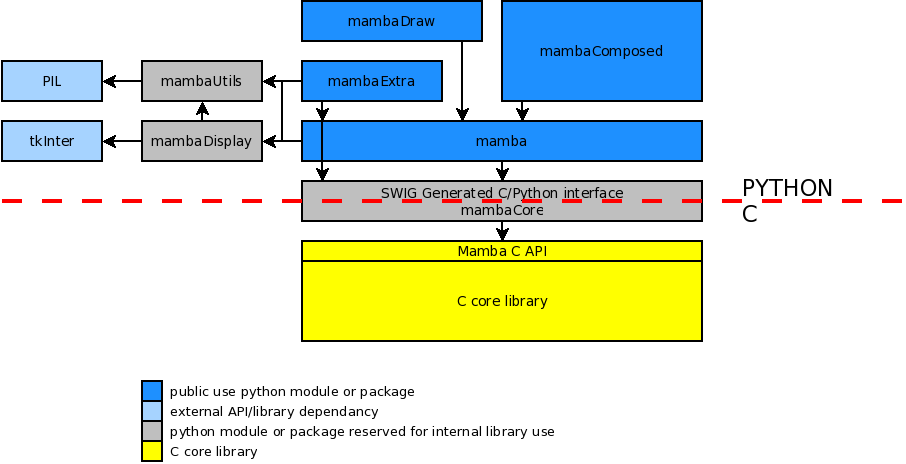
\includegraphics[scale=0.5]{archi.png}
\caption{Library architecture layout}
\label{fig:archi_lay}
\end{figure}

As you already know, Mamba is programmed in C and Python. The C code implements
very basic functions. They are coded to be specific, fast and simple. Each 
function performs only one operation and do it the best it can. The C code is 
compiled to create the core library which is a collection of simple operations.

Simple Wrapper Interface Generator (SWIG) is used to create the interface 
between the C code and the Python code. This tool makes it easier to add new
functions inside the C part by automatically generating the Python wrapper
around it (Except for particular parameters).

The Python code is split into various modules and packages. At the base
of it is the mamba module. This module implements the imageMb class that is the
central data structure of the library. This class is an extended, more Python
friendly, version of the data structure used to represent image data inside the
C core library. The mamba module also wraps the core functions to simplify them
and make them compatible with the imageMb class.

Because the C core library does not offer functions to read image files, Mamba
relies on the Python Imaging Library (PIL) to do so. The mambaUtils module is
an interface to PIL that makes sure images are properly loaded and converted to 
a format that is compatible with Mamba internal data representation.

The display capability is implemented by module mambaDisplay which relies on
Tkinter for windows and widgets creation. This module also uses mambaUtils 
functions for image handling (like save or load) performed directly using
a contextual menu.

The mambaExtra module is built on top of the mamba module. It implements
functions or classes that are, as its name tells, extras to the library. This
module relies on PIL, Tkinter and Mamba because of the variety of "extra".

The mambaDraw module implements all the drawing functions that come with the
library. It relies only on functions and classes found in the mamba module.

The same goes for the mambaComposed package which is where all the basic
functions found in the mamba module are combined to create more elaborated
mathematical morphology operators. This package is divided into multiple
modules for the sake of readability (smaller files regrouping operators by
family).

This architecture is described in figure \ref{fig:archi_lay}.

\subsection{Creating your own display}
\label{cha:create_own_disp}

If your intent is to create your own display for Mamba image, you can create
a "displayer" class inheriting from the mambaDisplayer class described in the
mambaDisplay module. This class is actually an abstract class (or as close
as an abstract class that is allowed by Python). The mambaDisplay module
actually implements one child class of the mambaDisplayer called \_MbDisplayer.
Creating your own display will then look like this:

\lstset{language=Python}
\begin{lstlisting}
import mambaDisplay

# your own displayer (inherits from the generic displayer)
class YourOwnDisplayer(mambaDisplay.mambaDisplayer):
    ...
    
# Creating an instance of your displayer
your_displayer = YourOwnDisplayer()

# Creating an image using your own display rather than the default one
im = imageMb(displayer=your_displayer)

# Or alternatively you could override the getDisplayer function of the 
# mambaDisplay module so that every created image will then use your display
# without having to precise it
def getDisplayer():
    global your_displayer
    return your_displayer
\end{lstlisting}

A "displayer" must implement various functionnalities to work correctly. The 
best way to create your own is to have a look at the default one in mambaDisplay.

\pagebreak

\appendix
\section{Examples}
\label{cha:examples}

This section presents some examples that you can retrieve in the examples
directory of the source files.

There are three types of examples :
\begin{enumerate}
\item \textbf{easy}: These are mainly intended for beginners so they could refer
to some basic examples to start their own code.
\item \textbf{moderate}: In these examples, more elaborated actions are performed
and presented. They cover usage that may not be difficult to do provided that you
read the documentation, but are more easily explained and understood with an
example.
\item \textbf{advanced}: These are more complex examples that should be considered
as demonstrators of the capabilities of the Mamba library.
\end{enumerate}

\begin{warnBox}
Examples presented here may not correctly work. We tried to put a wide range of
examples and produced this small selection after some efforts (some of them are
non-trivial) but we may have broke them in the process of publishing them. If
it so happens, try to see this as an exercise or e-mail us.
\end{warnBox}

\pagebreak

\input{examples}

\pagebreak

\section{To go further}
\label{cha:to_go_further}
\subsection{Python websites}

Here is a list of Python related websites:

\begin{itemize}
\item \url{http://www.python.org}: The official Python website. You can download
it there, find documentation and other links for Python.
\item \url{http://docs.python.org/tutorial/}: The official Python tutorial.
\item \url{http://www.greenteapress.com/thinkpython/thinkCSpy/}: How to Think 
Like a Computer Scientist. A free book to learn computer science with Python
programming. Many translation are available.
\item \url{http://www.pythonware.com/products/pil/}: The Python Imaging Library
website. You can download it, find documentation and source.
\item \url{http://wiki.python.org/moin/TkInter}: A wiki providing ressources
for the Tkinter library used in Mamba for display.
\item \url{http://www.pythonchallenge.com/}: An online puzzle game where you
will need to use Python to solve the riddles.
\end{itemize}

\subsection{Mathematical Morphology websites}

The list below presents websites where you will find courses, documentation and
other information related to mathematical morphology at large:

\begin{itemize}
\item \url{http://cmm.ensmp.fr/}: The Centre de Morphologie Math\'{e}matique
website. This Mines Paristech research laboratory was founded by Georges Matheron 
and Jean Serra, the pioneers of mathematical
morphology. Various publications are available with online courses.
\item \url{http://en.wikipedia.org/wiki/Mathematical_morphology}: The Wikipedia
page on mathematical morphology.
\end{itemize}

\subsection{Other mathematical morphology libraries}

If you are not happy with Mamba, here is a list of other mathematical morphology
libraries:

\begin{itemize}
\item \textsc{\textbf{Fulguro}}: A free library, released under LGPL, implementing
mathematical morphology and images processing functions. Coded in C with wrappers
for Python and Ruby. You can find it at \url{http://fulguro.sourceforge.net/}.
\item \textsc{\textbf{Morph-M}}: A proprietary library developed by the Centre
de Morphologie Math\'{e}matique. Morph-M is coded in C++ with a wrapper for
Python. More information can be found at \url{http://cmm.ensmp.fr/Morph-M/index_en.html}.
\end{itemize}

\end{document}
